\documentclass{article}
\usepackage{amsmath, amssymb, tikz, marvosym, tcolorbox, array, sfmath, enumerate, multicol, pgfplots}
\renewcommand{\familydefault}{\sfdefault}
\pgfplotsset{compat=newest}
\usetikzlibrary{arrows.meta}
\everymath{\displaystyle}
\tikzset{>=stealth}
\tikzstyle{input} = [circle, text centered, radius = 1cm, draw = black]
\tikzstyle{function} = [rectangle, text centered, minimum width = 2cm, minimum height = 1cm, draw = black]
\usepackage[top = 0.25in, bottom = 0.25in, left = 1in, right = 1in]{geometry}
\pagestyle{empty}
\raggedright

\newcounter{example}[section]
\newenvironment{example}[1][]{\refstepcounter{example}\par\medskip
   {\color{red}\textbf{Example~\theexample. #1}}}{\medskip}

\begin{document}

\section*{Composition of Functions}

\begin{tcolorbox}[colframe=orange!70!white, coltitle=black, title=\textbf{Summary}]
\begin{enumerate}
    \item With compositions of functions, the output of one function is used as input into the other.
    \item You can even evaluate entire functions into other functions.
\end{enumerate}
\end{tcolorbox}
\bigskip 

Compositions of functions involve {\color{blue}\textbf{substituting}} one function into the variable(s) of another.	\newline\\	

The composition of a function $f$ and $g$ denoted
\[ (f \circ g)(x) \]
\begin{center} is \end{center}
\[(f \circ g)(x) = f(g(x)) \]
\smallskip 

where we plug $g(x)$ into the variable for $f(x)$.	
\bigskip 

In other words, the output of $g(x)$ becomes the \textbf{input} of $f(x)$.
\vspace{0.25in}

The following illustrates finding $(f \circ g)(8)$, or $f(g(8))$, in which 
\[g(x)=2x+3 \text{ and } f(x) = x^2\]:		
\vspace{-12pt}

\begin{enumerate}
\item Evaluate $g(8)$ to get $2(8)+3$, or 19. 
\item Evaluate $f(19)$ to get $19^2$, or 361.
\end{enumerate}

\begin{center}
    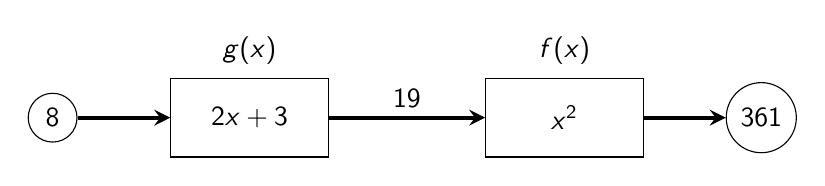
\begin{tikzpicture}[node distance = 2.5cm]
    \node (inputVal) [input] {8};
    \node (fx) [function, right of = inputVal] {$2x + 3$};
    \node (gx) [function, right of = fx, node distance = 4cm] {$x^2$};
    \node (outputVal) [input, right of = gx] {361};
    \node at (4.5,0) [anchor = south] {19};
    \node at (2.5,0.85) {$g(x)$};
    \node at (6.5,0.85) {$f(x)$};
    \draw [->, >=stealth, line width = 1.5] (inputVal) -- (fx);
    \draw [->, >=stealth, line width = 1.5] (fx) -- (gx);
    \draw [->, >=stealth, line width = 1.5] (gx) -- (outputVal);
    \end{tikzpicture}
\end{center}
\vspace{1in}

\begin{example}
Find each of the following if $f(x) = 3x-4$ and $g(x) = x^2 + 6$
\begin{multicols}{3}
\begin{enumerate}[(a)]
    \item $(f \circ g)(2)$
    \item $(g \circ f)(2)$
    \item $(f \circ f)(1)$
\end{enumerate}
\end{multicols}
\end{example}
\vfill 
\newpage 

We can even substitute an entire function into another and simplify.	
\bigskip 

Using $\color{red}g(x)=2x+3$ and $\color{blue}f(x)=x^2$, the composition $(f \circ g)(x)$ becomes
\begin{align*}
({\color{blue}f} \circ {\color{red}g})(x) &= {\color{blue}f}({\color{red}2x+3}) \\
&=({\color{red}2x+3})^2 \\
&=(2x+3)(2x+3) \\
&=\boxed{4x^2 + 12x + 9}
\end{align*}
\vspace{0.5in}

\begin{example}
Find each of the following if $f(x) = 3x-4$ and $g(x)=x^2+6$
\begin{enumerate}[(a)]
\begin{multicols}{2}
    \item $(f \circ g)(x)$
    \item $(g \circ f)(x)$
\end{multicols}
\vfill 
    \item $(f \circ f)(x)$
\end{enumerate}
\end{example}
\vfill 
\newpage

\subsection*{Tabular and Visual Methods}
\bigskip 

Remember, $f(x)$ tells you the output (or $y$-coordinate) of the function when plugging in a value for $x$. \newline\\

For instance, $f(3) = -2$ means
\begin{itemize}
    \item When the input is 3, the output is $-2$
    \item The point $(3,-2)$ is on the graph of the function.
\end{itemize}
\bigskip 

\begin{example} 
Find each given the table below.
\begin{center}
\begin{tabular}{c|c|c|c|c|c|c|c}
    $\pmb{x}$ & $\pmb{-3}$ & $\pmb{-2}$ & $\pmb{-1}$ & \textbf{0} & \textbf{1} & \textbf{2} & \textbf{3} \\ \hline 
    $\pmb{f(x)}$ & 1 & $-2$ & $-3$ & $-1$ & 3 & 2 & 0 \\ \hline
    $\pmb{g(x)}$ & $-2$ & 2 & $-3$ & 3 & 0 & 1 & $-1$ \\
\end{tabular}
\end{center}
\begin{multicols}{4}
\begin{enumerate}[(a)]
    \item $(f \circ g)(-1)$
    \item $f(g(2))$
    \item $(g \circ f)(0)$
    \item $g(g(-3))$
\end{enumerate}
\end{multicols}
\end{example}
\vfill 
\begin{example}
Find each given the graph below.
\begin{center}
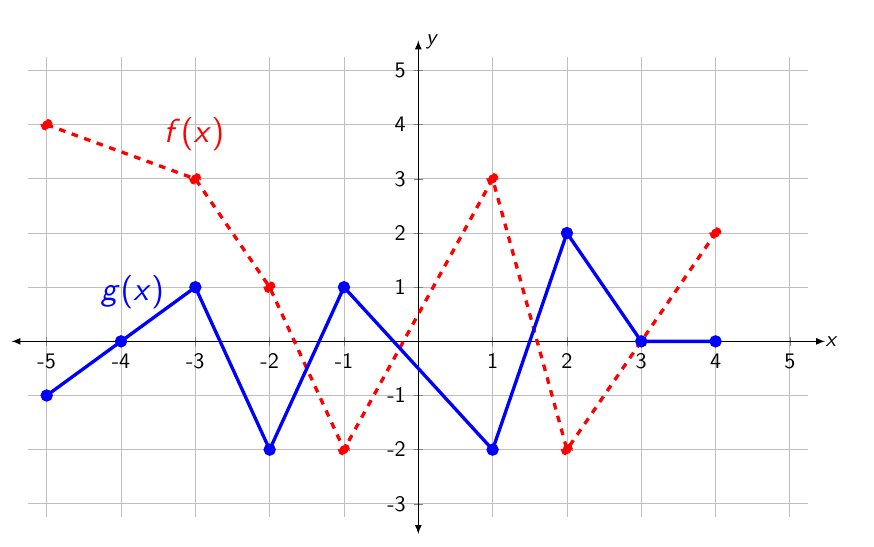
\begin{tikzpicture}[scale=0.8]
\begin{axis}
[   
    grid,
    axis lines=middle,
    xmin=-5.25,xmax=5.25,
    ymin=-3.25,ymax=5.25,
    restrict y to domain=-3:5,
    xtick={-5,-4,...,5},
    xticklabels={-5,-4,-3,-2,-1,,1,2,3,4,5},
    ytick={-3,-2,...,5},
    yticklabels={-3,-2,-1,,1,2,3,4,5},
    axis line style={latex-latex},
    axis line style={shorten >=-7.5pt, shorten <=-7.5pt},
    xlabel=$x$,
    ylabel=$y$,
    xlabel style={at={(ticklabel* cs:1)},anchor=west, xshift=0.15cm},
    ylabel style={at={(ticklabel* cs:1)},anchor=south west},
    width=5.5in,
    height=3.5in
]
\addplot[mark = *, color=red, line width = 1.5, dashed] coordinates
{
    (-5,4)
    (-3,3)
    (-2,1)
    (-1,-2)
    (1,3)
    (2,-2)
    (4,2)
};
\addplot[mark=*, color=blue, line width = 1.5] coordinates
{
    (-5,-1)
    (-4,0)  
    (-3,1)
    (-2,-2)
    (-1,1)
    (1,-2)
    (2,2)
    (3,0)
    (4,0)
};
\end{axis}
\node at (2.0,6.5) [anchor = north west] {\color{red} \large $f(x)$};
\node at (1,4) [anchor = north west] {\color{blue} \large $g(x)$};
\end{tikzpicture}
\end{center}
\begin{multicols}{4}
\begin{enumerate}[(a)]
    \item $(f \circ g)(-5)$
    \item $g(f(-2))$
    \item $f(f(2))$
    \item $(g \circ g)(-4)$
\end{enumerate}
\end{multicols}
\end{example}
\vfill 
\end{document}
